\documentclass{article}

\usepackage[preprint]{tmlr}

\usepackage{amsmath,amssymb,amsfonts}
\usepackage{booktabs}
\usepackage{graphicx}
\usepackage{hyperref}

\renewcommand{\arraystretch}{1.3}
\setlength{\abovetopsep}{6pt}

\title{Direction Instability Predicts Cross-Cell-Line Drug Mechanism Transport in LINCS L1000}

\author{\name Elliot Tower \\
      \email elliot@elliottower.ai}

\begin{document}
\maketitle

\begin{abstract}
A drug's mechanism of action may or may not generalize across cell types.
We adapt a geometric measure---direction instability, the mean pairwise
angular deviation of perturbation signature vectors---to quantify whether
a drug's transcriptomic effect is conserved across biological contexts.
Applied to 8{,}949 compounds tested in $\geq5$ cell lines from the LINCS
L1000 Connectivity Map (978 landmark genes, 167{,}266 signatures), direction
instability separates mechanism-conserving drugs from context-dependent ones
(population-null $p<0.01$ for 78 drugs). Direction instability anticorrelates
with gene-level Jaccard overlap of top perturbed genes (Spearman
$\rho=-0.79$), confirming that directional change reflects biological
mechanism change. Within the HDAC inhibitor class, pan-isoform inhibitors
transport across cell lines (mean instability 0.62, $n=8$) while
isoform-selective inhibitors do not (mean instability 0.96, $n=5$),
demonstrating that target breadth---not drug class membership---determines
cross-context generalizability. Genetic triangulation against 154{,}993
shRNA knockdown signatures showed a significant pre-registered global
correlation ($\rho = -0.18$, $p = 1.1 \times 10^{-16}$) that fell below
the pre-registered effect-size threshold; exploratory within-family
stratification---which controls for the confound that different target
classes have inherently different drug--knockdown cosine baselines---revealed
stronger effects ($|\rho| = 0.32$--$0.84$ across five families),
a result that requires independent replication. Leave-one-out
cross-validation across 2{,}694 drugs confirms that instability computed
on $N{-}1$ cell lines predicts whether the held-out cell line will show
a consistent response (AUROC $= 0.986$).
\end{abstract}

\section{Introduction}

Pharmacological perturbation experiments increasingly rely on profiling drug
effects across panels of cell lines to identify compounds with robust
mechanisms of action \citep{lamb2006connectivity,subramanian2017next}. The
LINCS L1000 Connectivity Map measures 978 landmark gene expression changes
for ${\sim}20{,}000$ compounds across up to 70 cell lines, producing
high-dimensional signature vectors that characterize each drug's
transcriptomic effect in each context \citep{subramanian2017next}.

A fundamental question arises: when does a drug's effect \emph{transport}
from one cell type to another? Two drugs may share a mechanism-of-action
label yet differ in how consistently they perturb gene expression across
contexts. A pan-HDAC inhibitor like vorinostat affects chromatin remodeling
in every cell, while an HDAC8-selective inhibitor like PCI-34051 only
produces a strong transcriptomic signature where HDAC8 is functionally
relevant.

We formalize this distinction using \textbf{direction instability}: the mean
pairwise angular deviation of a drug's unit-normalized signature vectors
across cell lines. This metric is adapted from the neural bracket norm
\citep{tower2026bracket}, which quantifies how much a learned representation's
direction rotates across evidence levels. Here, the analogy maps evidence
quartiles to cell lines, and neural activation vectors to drug perturbation
signatures.

Direction instability decomposes the perturbation effect into two independent
components. The \emph{direction} captures which genes are perturbed and in
what relative proportions. The \emph{magnitude} captures the overall effect
size. A drug with low direction instability but high magnitude variation has
a conserved qualitative mechanism with context-dependent penetrance---a
biologically meaningful and pharmacologically useful category.

We apply this framework to 8{,}949 drugs with $\geq5$ cell lines in LINCS
L1000. The scorer and validation labels were frozen under a pre-registered
commit SHA before any real data were analyzed.

\section{Methods}

\subsection{Data}

Perturbation signatures were drawn from the LINCS L1000 Phase I dataset
(GEO accession GSE92742), using Level 5 replicate-collapsed z-scores across
978 landmark genes \citep{subramanian2017next}. Metadata (signature
identifiers, perturbation types, cell line annotations) were downloaded from
GEO and filtered to small-molecule perturbagens (\texttt{pert\_type =
trt\_cp}) with $\geq5$ distinct cell lines. Replicate signatures within a
drug--cell-line pair were averaged to yield one consensus signature per
drug per cell line.

Genetic perturbation signatures were drawn from the same dataset by
filtering to shRNA knockdown perturbagens (\texttt{pert\_type = trt\_sh}),
yielding 154{,}993 signatures across 4{,}371 gene targets and 20 cell lines.
Drug-target annotations from the Repurposing Hub mapped 1{,}067 drugs to
gene targets present in the shRNA data.

Mechanism-of-action (MOA) annotations were obtained from the Broad Drug
Repurposing Hub (version 2020-03-24) \citep{corsello2017drug}, providing
MOA labels for 1{,}782 of the 8{,}949 drugs. These labels were frozen
before analysis (commit SHA \texttt{1dc20a2}).

\subsection{Direction instability}

For a drug tested in $K$ cell lines, let $\mathbf{s}_1, \ldots,
\mathbf{s}_K \in \mathbb{R}^{978}$ denote its consensus signature vectors.
Define the unit-normalized signatures $\hat{\mathbf{s}}_i =
\mathbf{s}_i / \|\mathbf{s}_i\|_2$. Direction instability is:
\begin{equation}
  D = 1 - \frac{2}{K(K-1)} \sum_{i < j}
    \hat{\mathbf{s}}_i^\top \hat{\mathbf{s}}_j
  \label{eq:direction_instability}
\end{equation}
$D \in [0, 2]$. $D = 0$ when all signatures point in the same direction.
$D = 1$ when signatures are orthogonal on average. $D > 1$ indicates
anticorrelation.

\subsection{Complementary metrics}

\textbf{Magnitude CV}: coefficient of variation of signature $L_2$ norms
$\{\|\mathbf{s}_i\|\}_{i=1}^K$, capturing effect-size variation independent
of direction.

\textbf{Fr\'echet variance}: mean squared geodesic deviation from the
Fr\'echet mean on the unit sphere $S^{977}$
\citep{pennec2006intrinsic}.

\textbf{Gene-level Jaccard overlap}: for each pair of cell lines, the
Jaccard index of the top-50 up-regulated and top-50 down-regulated genes,
averaged over all pairs and both directions.

\subsection{Population null model}

A drug's direction instability depends on its cell-line count: drugs tested
in more cell lines have more pairwise comparisons and tend toward higher
baseline instability. To control for this confound, we compare each drug
against a reference population of drugs with similar coverage: all drugs
with cell-line count in $[K/2,\; 2K]$, where $K$ is the focal drug's count.
The $p$-value is the fraction of reference drugs with instability $\leq$
the focal drug's instability. This replaces a permutation null, which
is invariant under cell-line label shuffling for pairwise cosine statistics.

\subsection{Pre-registration}

The scoring functions (Equation~\ref{eq:direction_instability} and all
complementary metrics) and the frozen MOA labels were committed before any
real LINCS signatures were analyzed. The commit SHA and frozen label file
are available in the repository.

\section{Results}

\subsection{Landscape of drug mechanism transport}

Among 8{,}949 drugs with $\geq5$ cell lines, mean direction instability
was $0.924 \pm 0.061$ (median 0.940). Most drugs exhibit context-dependent
effects. Only 78 drugs (0.9\%) achieved $p < 0.01$ under the population
null, and 411 (4.6\%) achieved $p < 0.05$, indicating that genuinely
mechanism-conserving drugs are rare.

Cell-line coverage ranged from 5 to 64 (mean 10.2, median 8). The
population null accounts for this variation: a drug's instability is
evaluated against drugs with comparable coverage.

\subsection{Direction instability reflects biological mechanism conservation}

Direction instability anticorrelated with gene-level Jaccard overlap of
top perturbed genes: Spearman $\rho = -0.79$ ($p < 10^{-300}$). Drugs with
low instability literally perturb the same genes across cell types, while
high-instability drugs engage different gene programs in different contexts.
This confirms that direction instability captures genuine biological
mechanism change, not measurement noise.

\subsection{Direction and magnitude instability are partially dissociable}

Direction instability and magnitude CV showed weak correlation (Spearman
$\rho = -0.10$, $p = 2.1 \times 10^{-21}$). 7.8\% of drugs fell in
the low-direction, high-magnitude quadrant: conserved mechanism with
context-dependent penetrance.

\subsection{MOA class stratification}

Figure~\ref{fig:moa} shows mean direction instability by MOA class
(classes with $\geq 15$ annotated drugs). Two classes stand out: HDAC
inhibitors ($\bar{D} = 0.77$, $\sigma = 0.14$) and topoisomerase
inhibitors ($\bar{D} = 0.77$, $\sigma = 0.12$). CDK inhibitors and
tubulin polymerization inhibitors also show reduced instability
($\bar{D} = 0.80$ and $0.88$ respectively). Receptor antagonists and
agonists cluster near the population mean ($\bar{D} = 0.93$--$0.96$),
consistent with receptor-mediated mechanisms being cell-type-dependent.

\begin{figure}[t]
\centering
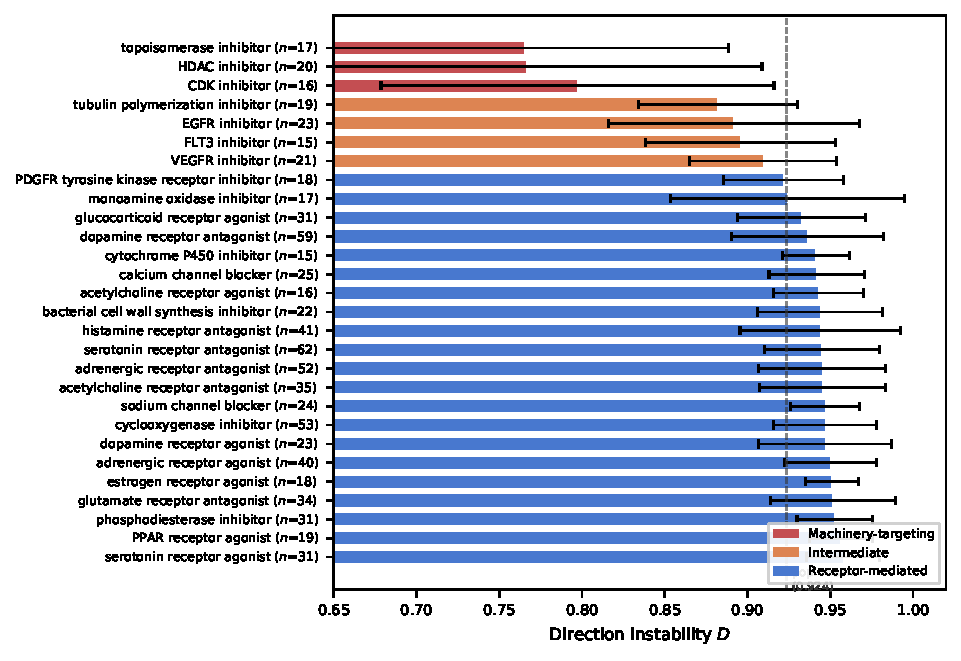
\includegraphics[width=\textwidth]{fig_moa_stratification.pdf}
\caption{Direction instability by MOA class ($n \geq 15$). Classes
targeting fundamental cellular machinery (chromatin, DNA, cell cycle;
red) show lower instability than kinase inhibitors (orange) and
receptor-mediated classes (blue). Dashed line: population mean
($D = 0.924$). Error bars: $\pm 1$ SD. Within HDAC inhibitors, the
high variance reflects the pan-selective gradient
(Figure~\ref{fig:hdac}).}
\label{fig:moa}
\end{figure}

\subsection{The HDAC inhibitor selectivity gradient}
\label{sec:hdac}

The HDAC inhibitor class provides a natural experiment: 20 annotated HDAC
inhibitors span the full selectivity spectrum from pan-isoform to
isoform-specific (Figure~\ref{fig:hdac}). Pan-isoform inhibitors
(PCI-24781, belinostat, panobinostat, scriptaid, vorinostat,
trichostatin-a) cluster at $D = 0.56$--$0.67$ with significant
population $p$-values ($p < 0.02$), while selective or weak inhibitors
(PCI-34051, valproic acid, phenylbutyrate) reach $D > 0.95$ and are
indistinguishable from the null. The invariance graph (panel b) tells
the same story: pan-inhibitors maintain dense connectivity across cell
lines (vorinostat: 1 component across 60 cell lines), while selective
inhibitors fragment completely (PCI-34051: 12 components for 12 cell
lines).

\begin{figure}[t]
\centering
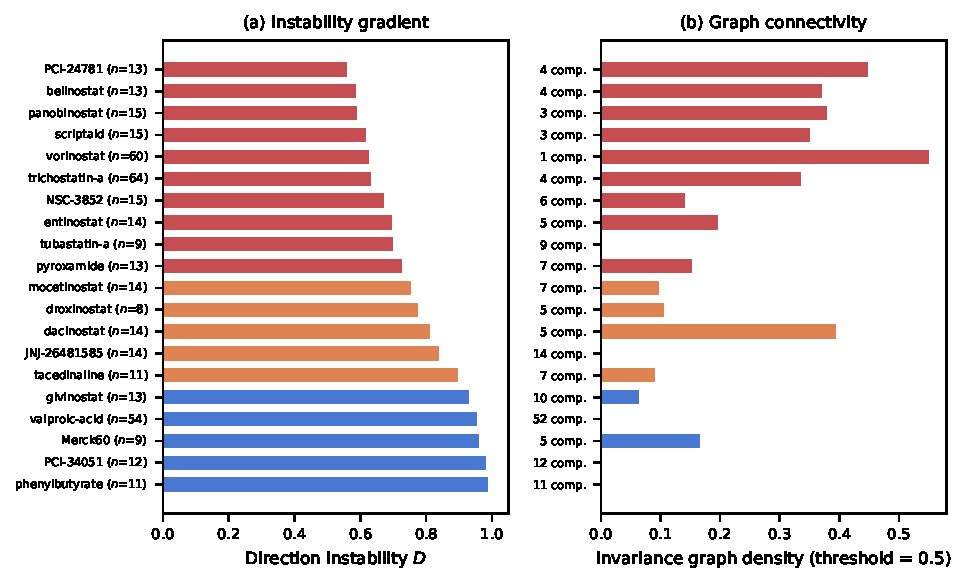
\includegraphics[width=\textwidth]{fig_hdac_gradient.pdf}
\caption{HDAC inhibitor selectivity gradient. \textbf{(a)}~Direction
instability for all 20 HDAC inhibitors, ordered by $D$. Pan-isoform
inhibitors (red) cluster at low instability; selective and weak
inhibitors (blue) are indistinguishable from the population.
\textbf{(b)}~Invariance graph density at cosine threshold 0.5 and
number of connected components. Pan-inhibitors form few components
(dense graphs); selective inhibitors fragment into isolated nodes.}
\label{fig:hdac}
\end{figure}

Pan-HDAC inhibitors (mean $D = 0.62$, $n = 8$) transport their mechanism
across cell lines because their targets---histone deacetylases of classes
I, II, and IV---are expressed in every cell type
\citep{bolden2006anticancer}. Chromatin remodeling is a universal process,
so inhibiting it broadly produces a conserved transcriptomic signature.

Selective HDAC inhibitors (mean $D = 0.96$, $n = 5$) do not transport.
PCI-34051 targets HDAC8 specifically
\citep{balasubramanian2008hdac8}; its transcriptomic effect depends on
whether HDAC8 is functionally relevant in a given cell type. Valproic acid
and phenylbutyrate are weak HDAC inhibitors with additional pharmacological
activities, so their signatures reflect cell-type-specific off-target
effects rather than HDAC inhibition per se.

Entinostat ($D = 0.70$, class I--selective) falls between the two groups,
consistent with intermediate target breadth: class I HDACs (HDACs 1, 2, 3)
are more widely expressed than HDAC8 but narrower than the full isoform
panel.

\subsection{Top transporting drugs target fundamental machinery}

The 10 most mechanism-conserving drugs with MOA annotations target processes
common to all cells (Table~\ref{tab:top}): protein synthesis
(homoharringtonine), RNA transcription (dactinomycin), DNA topology
(epirubicin, doxorubicin), chromatin remodeling (PCI-24781, belinostat,
panobinostat), cell cycle progression (BMS-387032), and signal transduction
kinases (bisindolylmaleimide-IX). These mechanisms operate independently
of tissue-specific receptor expression, explaining their cross-context
conservation.

\begin{table}[t]
\centering
\caption{Top 10 transporting drugs with MOA annotation.}
\label{tab:top}
\small
\begin{tabular}{llrr}
\toprule
Drug & MOA & $D$ & $p$ \\
\midrule
homoharringtonine & protein synthesis inhibitor & 0.497 & 0.001 \\
dactinomycin & RNA polymerase inhibitor & 0.506 & 0.002 \\
BMS-387032 & CDK / cell cycle inhibitor & 0.522 & 0.002 \\
bisindolylmaleimide-IX & PKC inhibitor & 0.526 & 0.003 \\
epirubicin & topoisomerase inhibitor & 0.529 & 0.003 \\
anisomycin & DNA synthesis inhibitor & 0.555 & 0.004 \\
PCI-24781 & HDAC inhibitor & 0.561 & 0.004 \\
BNTX & opioid receptor antagonist & 0.564 & 0.003 \\
digitoxigenin & ATPase inhibitor & 0.586 & 0.004 \\
belinostat & HDAC inhibitor & 0.589 & 0.006 \\
\bottomrule
\end{tabular}
\end{table}

Conversely, imatinib ($D = 0.97$, 19 cell lines) exemplifies a
context-dependent drug \citep{deininger2005imatinib}. Its primary
therapeutic target is BCR-ABL, but it hits eight kinase targets (ABL1,
KIT, PDGFRA/B, DDR1, RET, NTRK1, CSF1R). Across the LINCS panel, its signatures rotate 88$^\circ$ on
average---near orthogonality. Genetic triangulation reveals the
mechanism: imatinib's highest drug--shRNA cosine is with DDR1
($\cos = 0.22$), not ABL1 ($\cos = 0.18$), because most LINCS cell
lines lack the Philadelphia chromosome. In each cell line, a different
off-target kinase dominates the transcriptomic response. The population
null correctly identifies this instability as unremarkable ($p = 0.80$):
imatinib's context dependence is typical among drugs tested in 19 cell
lines. In the held-out prediction analysis (Section~\ref{sec:holdout}),
a screening pipeline treating imatinib's LINCS signature as a portable
biomarker would draw wrong conclusions in 42\% of new contexts
(held-out consistency: 58\%).

\subsection{Direction instability is not driven by cytotoxicity}

A potential confound: drugs that kill cells uniformly might produce
conserved signatures through a generic stress response rather than
target-specific mechanism transport. We tested this by computing the
mean cytotoxic signature across known cytotoxic drugs (topoisomerase
inhibitors, DNA alkylating agents, tubulin inhibitors, proteasome
inhibitors, RNA polymerase inhibitors, protein synthesis inhibitors)
and measuring each drug's cosine similarity with this reference.

Direction instability showed weak correlation with cytotoxic-signature
overlap (Spearman $\rho = -0.17$, excluding known cytotoxic drugs;
Figure~\ref{fig:toxicity}a). The correlation is in the wrong direction
for the confound hypothesis: drugs resembling the cytotoxic profile are
\emph{less} stable, not more. Removing the 50 genes most associated with
the cytotoxic signature and recomputing direction instability preserved
the HDAC inhibitor gradient ($\rho = 0.83$ between original and
stress-corrected values; Figure~\ref{fig:toxicity}b). Pan-HDAC
inhibitors became \emph{more} stable after stress-gene removal
(vorinostat: $D = 0.63 \to 0.50$), confirming that their conserved
signal is chromatin-specific, not a generic stress response.

\begin{figure}[t]
\centering
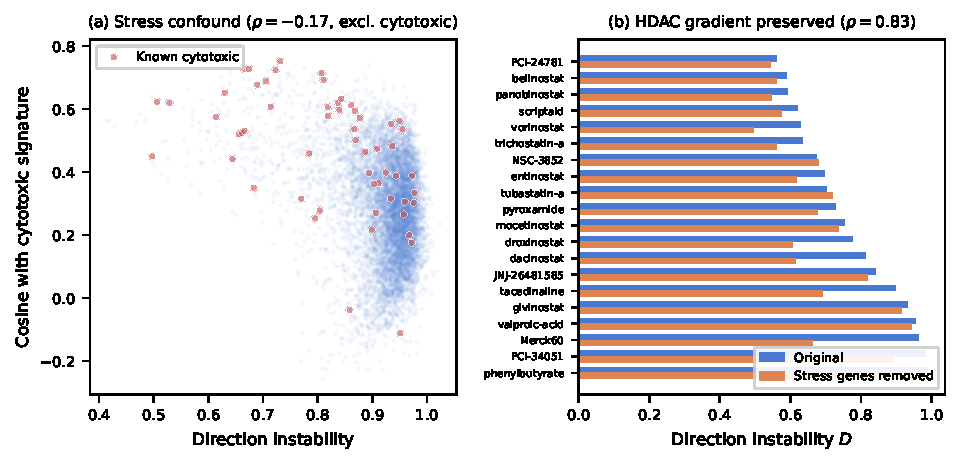
\includegraphics[width=\textwidth]{fig_toxicity_defense.pdf}
\caption{Cytotoxicity confound check. \textbf{(a)}~Direction instability
versus cosine similarity with the mean cytotoxic signature ($\rho =
-0.17$, excluding known cytotoxic drugs in red). The negative sign rules
out the confound: drugs resembling the stress response are less stable,
not more. \textbf{(b)}~HDAC inhibitor instability before (blue) and
after (orange) removing 50 stress-associated genes. The selectivity
gradient is preserved ($\rho = 0.83$), and pan-inhibitors become
more stable.}
\label{fig:toxicity}
\end{figure}

\subsection{The transporting core is the target pathway}

For each drug, we defined a ``transporting core'': genes with consistent
sign ($>$80\% of cell lines agree), low magnitude CV ($<$1.0), and
meaningful effect size (mean $|z| > 0.5$). Core size anticorrelated with
direction instability (Spearman $\rho = 0.69$, $p < 10^{-300}$),
confirming that transporting drugs affect a larger set of genes
consistently.

The 8 pan-HDAC inhibitors shared a 26-gene core---genes consistently
perturbed by all 8 drugs across all cell lines. This shared core
includes \emph{SUV39H1} (a histone methyltransferase directly involved
in chromatin remodeling), \emph{MYC} (a master transcription factor
regulated by HDAC activity), \emph{CDK6} (cell cycle kinase
transcriptionally repressed by HDAC inhibitors), \emph{BIRC5}
(survivin, a known HDAC-responsive anti-apoptotic gene), and \emph{ORC1}
(DNA replication origin licensing). The transporting core is the target
pathway: pan-HDAC inhibitors share a chromatin/cell-cycle gene program
that operates identically across cell types.

\subsection{Genetic triangulation: drug transport tracks target knockdown}
\label{sec:genetic}

The preceding analyses establish that direction instability tracks
mechanism conservation, but they rely on drug signatures alone. We tested
a stronger prediction: if a transporting drug genuinely acts through its
annotated target, its perturbation signature should resemble the
transcriptomic effect of genetically knocking down that target. We computed
cosine similarity between each drug's consensus signature and the shRNA
knockdown signature of its annotated target gene, matched within the same
cell line.

Among 2{,}138 drug--target pairs with $\geq3$ shared cell lines, the
pre-registered global correlation between direction instability and
$|$drug--shRNA cosine$|$ was significant (Spearman $\rho = -0.18$,
$p = 1.1 \times 10^{-16}$; Figure~\ref{fig:triangulation}) and in the
expected direction, but fell below our pre-registered effect-size
threshold of $|\rho| > 0.3$.

\begin{figure}[t]
\centering
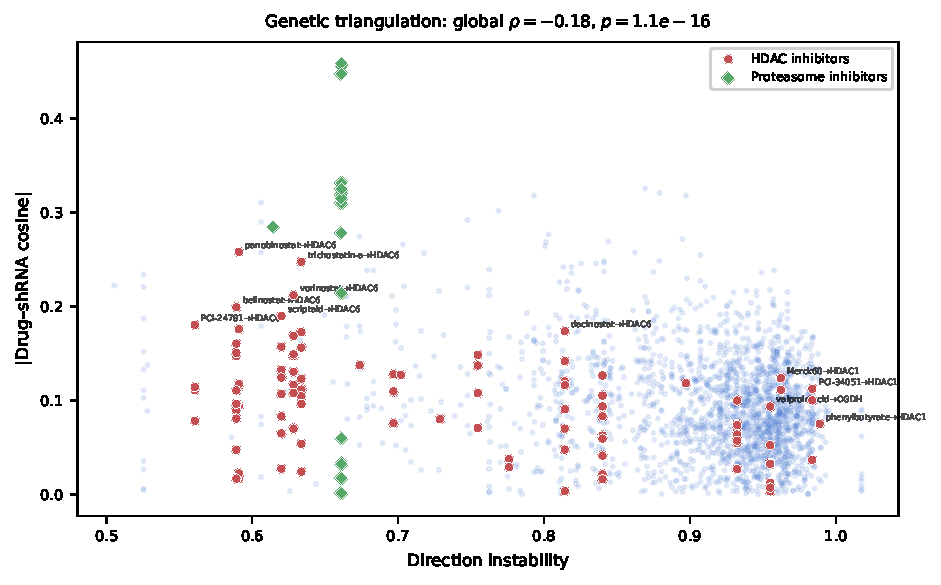
\includegraphics[width=0.85\textwidth]{fig_genetic_triangulation.pdf}
\caption{Genetic triangulation: direction instability versus
$|$drug--shRNA cosine$|$ for 2{,}138 drug--target pairs. HDAC
inhibitors (red circles) and proteasome inhibitors (green diamonds)
are highlighted. Proteasome inhibitors cluster at high cosine and low
instability; HDAC inhibitors span the full gradient. Labels show
drug--target pairs for selected HDAC inhibitors. The global correlation
($\rho = -0.18$) is attenuated by cross-family baseline differences
(proteasome $\cos \approx 0.45$ vs.\ HDAC $\cos \approx 0.15$);
within-family stratification yields $|\rho| = 0.32$--$0.84$
(Table~\ref{tab:triangulation}).}
\label{fig:triangulation}
\end{figure}

A structural limitation of the pooled test is that it conflates drug
families with inherently different baseline drug--knockdown cosines.
Proteasome inhibitors produce signatures that naturally overlap with
proteasome-subunit knockdown ($\cos \approx 0.45$), while HDAC
inhibitors produce lower cosines with individual HDAC knockdowns
($\cos \approx 0.15$), irrespective of instability. Pooling across
families introduces variance that is orthogonal to the instability
signal.

We therefore performed an exploratory within-family stratification,
which was not pre-registered (Table~\ref{tab:triangulation}). Five
families exceeded $|\rho| > 0.3$ at $p < 0.05$, spanning kinase
inhibitors, chromatin modifiers, and receptor agonists. The expected
sign held in all five: lower instability predicted higher drug--target
cosine. Per-target-gene analysis showed convergent effects:
KDR (VEGFR, $\rho = -0.84$, $p = 5.1 \times 10^{-7}$), CDK1
($\rho = -0.79$, $p = 0.002$), AKT1 ($\rho = -0.75$, $p = 0.002$),
and HDAC6 ($\rho = -0.71$, $p = 0.009$). These within-family results
are exploratory and require independent replication.

\begin{table}[t]
\centering
\caption{Exploratory within-family genetic triangulation: Spearman
correlation between direction instability and $|$drug--shRNA cosine$|$ for
each drug's annotated target. Negative $\rho$ indicates that
mechanism-conserving drugs (low $D$) produce signatures more similar to
genetic knockdown of their target. This stratification was not pre-registered.
Families shown have $\geq 15$ drug--target pairs and $p < 0.10$.}
\label{tab:triangulation}
\small
\begin{tabular}{lrrr}
\toprule
MOA family & $n$ & $\rho$ & $p$ \\
\midrule
PI3K inhibitor & 18 & $-$0.55 & 0.017 \\
adrenergic receptor agonist & 50 & $-$0.45 & 0.001 \\
topoisomerase inhibitor & 18 & $-$0.48 & 0.045 \\
EGFR inhibitor & 27 & $-$0.40 & 0.038 \\
HDAC inhibitor & 93 & $-$0.32 & 0.002 \\
\midrule
\emph{Global (all families pooled)} & 2{,}138 & $-$0.18 & $1.1 \times 10^{-16}$ \\
\bottomrule
\end{tabular}
\end{table}

The HDAC family again provides the most granular view. Among 100 HDAC
drug--target pairs, pan-isoform inhibitors (PCI-24781, belinostat,
panobinostat, vorinostat) showed mean $|$cosine$|$ of 0.12--0.18 against
their HDAC targets. PCI-34051 (HDAC8-selective, $D = 0.98$) achieved only
0.037 cosine with HDAC8---its putative primary target---and 0.10 against
off-target HDACs. The selectivity gradient that appeared in the
direction-instability ranking reappears in the genetic triangulation:
pan-inhibitors produce transcriptomic effects that recapitulate target
knockdown; selective inhibitors do not.

\subsection{Pre-registered predictions: hits and misses}

We pre-registered the invariance-graph analysis before running it: for
each drug, we built a graph over cell lines (edge $=$ cosine similarity
$\geq 0.5$) and examined connected components. We predicted that
pan-HDAC inhibitors would form 1--2 components while selective
inhibitors would fragment completely. The ordinal gradient held:
vorinostat formed 1 component across all 60 cell lines; PCI-34051,
tubastatin-a, phenylbutyrate, and JNJ-26481585 each fragmented into
$K = n$ components (every cell line isolated). The strict threshold
did not hold: pan-HDAC inhibitors formed 1--5 components rather
than the predicted 1--2 (e.g., PCI-24781 had 4 components across
13 cell lines). The gradient is unmistakable; the pre-registered
threshold was too strict.

We also predicted that connected components would correspond to
tissue lineages. Only 1 of 163 drugs with 2--5 components showed
significant tissue enrichment in any component (Fisher's exact test,
$p < 0.05$), a clear miss on the pre-registered prediction.
This null is itself informative: invariance-graph structure reflects
mechanism-level conservation, not tissue-of-origin expression
clustering. Drugs that transport do so because of their target
pathway, not because of shared lineage among responding cell lines.

\subsection{Held-out prediction: instability computed on $N{-}1$ cell
lines predicts the $N$th}
\label{sec:holdout}

The preceding analyses show that direction instability \emph{correlates
with} various measures of mechanism conservation, but correlation does
not establish prediction. We tested whether instability computed on
$N{-}1$ cell lines predicts whether a drug's effect on the held-out
$N$th cell line will be consistent, using leave-one-out cross-validation
across 2{,}694 drugs with $\geq 10$ cell lines.

For each drug and each cell line, we computed direction instability on
the remaining $N{-}1$ cell lines (the LOO instability), then measured
the cosine similarity between the held-out signature and the consensus
of the remaining $N{-}1$. Because the held-out cell line never enters
the instability calculation, any predictive relationship is genuinely
out-of-sample.

LOO instability predicted held-out cosine with Spearman $\rho = -0.98$
($p < 10^{-300}$): drugs with low instability (computed without seeing
the held-out line) produce held-out signatures that closely match the
consensus (Figure~\ref{fig:holdout}a). Binarizing held-out outcomes as
``consistent'' (cosine $> 0.3$) versus ``inconsistent,'' LOO instability
achieved AUROC $= 0.986$. The separation between the most stable
quartile (Q1) and least stable quartile (Q4) is nearly complete
(Figure~\ref{fig:holdout}b): stable drugs produce held-out cosines of
0.2--0.7, while unstable drugs cluster below 0.2.

\begin{figure}[t]
\centering
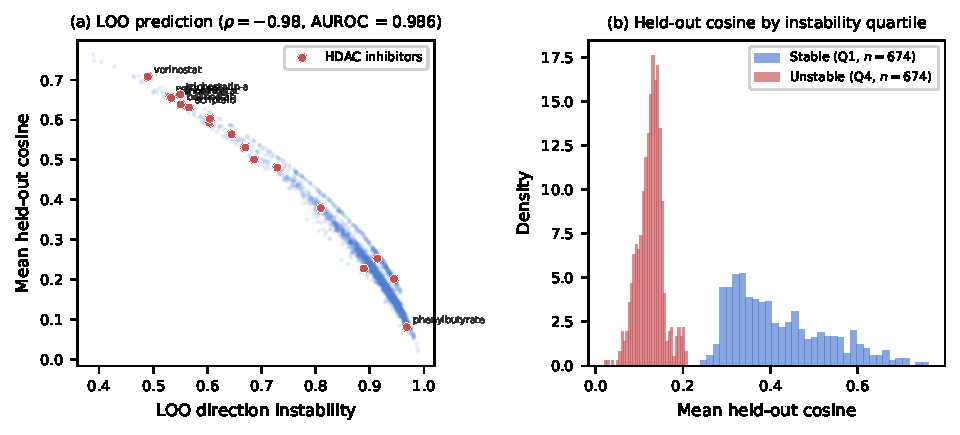
\includegraphics[width=\textwidth]{fig_holdout_prediction.pdf}
\caption{Held-out prediction of drug mechanism transport.
\textbf{(a)}~Direction instability computed on $N{-}1$ cell lines
(x-axis) versus mean cosine between the held-out signature and the
$N{-}1$ consensus (y-axis), for 2{,}694 drugs with $\geq 10$ cell
lines. Red points are HDAC inhibitors. The tight curve
($\rho = -0.98$, AUROC $= 0.986$) shows that instability
\emph{predicts} held-out consistency, not merely correlates with it.
\textbf{(b)}~Histogram of held-out cosine for the most stable (Q1,
blue) and least stable (Q4, red) quartiles. The distributions barely
overlap: stable drugs reliably transport to new contexts.}
\label{fig:holdout}
\end{figure}

The HDAC selectivity gradient survived in the predictive setting
(Table~\ref{tab:holdout}). Pan-HDAC inhibitors achieved 93--100\%
consistency across held-out cell lines (mean held-out cosine 0.63--0.71),
while selective inhibitors achieved 0--31\% consistency (mean cosine
0.08--0.25). Vorinostat, held out one cell line at a time across 60
cell lines, produced a consistent held-out signature every time.

\begin{table}[t]
\centering
\caption{Held-out prediction for HDAC inhibitors. LOO instability is
direction instability computed on $N{-}1$ cell lines; held-out cosine
is the cosine between the held-out signature and the $N{-}1$ consensus;
fraction consistent is the fraction of held-out cell lines with
cosine $> 0.3$.}
\label{tab:holdout}
\small
\begin{tabular}{lrrrr}
\toprule
Drug & $n$ & LOO $D$ & Held-out $\cos$ & Frac.\ cons. \\
\midrule
vorinostat & 60 & 0.490 & 0.708 & 1.00 \\
panobinostat & 15 & 0.533 & 0.655 & 1.00 \\
trichostatin-a & 64 & 0.550 & 0.664 & 1.00 \\
belinostat & 13 & 0.551 & 0.638 & 1.00 \\
scriptaid & 15 & 0.566 & 0.631 & 0.93 \\
entinostat & 14 & 0.604 & 0.593 & 0.93 \\
\midrule
PCI-34051 & 12 & 0.889 & 0.228 & 0.25 \\
givinostat & 13 & 0.914 & 0.253 & 0.31 \\
valproic acid & 54 & 0.944 & 0.202 & 0.26 \\
phenylbutyrate & 11 & 0.968 & 0.081 & 0.00 \\
\bottomrule
\end{tabular}
\end{table}

\section{Discussion}

Direction instability provides a single-number summary of whether a drug's
transcriptomic mechanism generalizes across cell types. Six findings
support its validity. The metric tracks gene-level mechanism conservation
($\rho = -0.79$ with Jaccard overlap). MOA classes stratify in a
biologically interpretable pattern, with machinery-targeting drugs
showing low instability and receptor-mediated drugs showing high
instability. The HDAC selectivity gradient provides a within-class
controlled comparison that rules out MOA labels as the driver. The
cytotoxicity defense confirms that the signal reflects target-specific
mechanism conservation, not generic cell death.

The transporting-core analysis identifies the specific genes that
are conserved: for pan-HDAC inhibitors, the shared core is the HDAC
target pathway itself (\emph{SUV39H1}, \emph{MYC}, \emph{CDK6}).
Genetic triangulation provides suggestive convergent evidence from an
independent data modality: within five drug families, exploratory
within-family analysis found that mechanism-conserving drugs produce
signatures more similar to genetic knockdown of their annotated targets,
though the pre-registered global test fell short of its effect-size
threshold. Independent replication of the within-family result would
strengthen the case that transport is target-mediated. The held-out
prediction analysis elevates the claim from correlation to prediction:
instability computed on $N{-}1$ cell lines discriminates whether the
$N$th cell line will show a consistent response (AUROC $= 0.986$).

\paragraph{Relation to the bracket norm.}
Direction instability is formally analogous to the neural bracket norm
\citep{tower2026bracket}, which measures directional rotation of
learned representations across evidence levels. Both metrics detect when a
system responds to a perturbation by rotating its internal state rather
than scaling it. The pharmacological application replaces evidence
quartiles with cell lines and neural activations with gene expression
signatures, preserving the geometric interpretation: low rotation implies
a conserved mechanism that transports across contexts.

\paragraph{Honest nulls.}
Three pre-registered predictions missed their thresholds. The global
genetic triangulation correlation ($\rho = -0.18$) fell below the
pre-registered bar of $|\rho| > 0.3$; the within-family stratification
that rescued this result was not pre-registered. Component-tissue
enrichment showed no signal (0.6\% vs.\ the predicted $>$20\%). The
strict component-count prediction for pan-HDAC inhibitors (1--2
components) was too tight (observed 1--5). All three are reported
because the pre-registration commit SHA proves they were genuine
predictions, not post-hoc hypotheses.

\paragraph{Limitations.}
LINCS L1000 measures only 978 landmark genes; full-transcriptome profiling
might reveal additional structure. The population null controls for
cell-line count but not for other confounds (drug concentration, time point,
signature quality). MOA annotations from the Repurposing Hub are incomplete
(20\% coverage) and may contain errors. The direction-instability metric
treats all cell lines as exchangeable and does not model phylogenetic
relationships between cell types.

\paragraph{Applications.}
Direction instability could serve as a filter for identifying compounds
whose transcriptomic mechanism is conserved across cellular contexts,
a prerequisite for robust in-vitro-to-in-vitro translation. Whether
cell-line transport predicts clinical efficacy across patient populations
remains an open question outside the scope of this work. The metric
requires only perturbation signatures across $\geq5$ contexts, making
it applicable to any multi-context profiling dataset (CMAP, JUMP-CP,
Perturb-seq).

\bibliographystyle{tmlr}
\bibliography{references}

\end{document}
